\documentclass[11pt, oneside]{article} 
\usepackage{preamble}
\usepackage{kpfonts}

\geometry{tmargin=.75in, bmargin=.75in, lmargin=.75in, rmargin = .75in}  

\title{\bf HOMOLOGICAL METHOD IN QUANTUM FIELD THEORY}
\author{SI LI \\ (\textit{Typeset by KEVIN LOO})}
\date{Spring 2022\\ (Updated \today)}

\begin{document}
\maketitle
\thispagestyle{empty}
\tableofcontents

\newpage
\setcounter{page}{1}

\section{Introduction}\label{sec:intro}
A physics system is always described by an action functional (if exist)
\bea
S: \sE \ra \bR,
\eea
where $\sE$ is the {\em space of fields}. In classical physics the variation of the action functional $S$ gives rise to the equations of motion, $\delta S=0$. These are described by the critical locus of the action functional:
\bea
\operatorname{Crit}(S)= \lcb \delta S=0\rcb / \sim,
\eea
which is a set of equivalence classes induced by arbitrary symmetry. In this lecture, we will focus on quantum physics. One convenient way to approach quantum physics is by {\bf Feynman path integral}
\bea
\int_\sE e^{iS/\hbar}\ .
\eea

\begin{eg} Here are some basic examples of quantum field theory that we will discuss
throughout this lecture.
\bi[(1)]
\item \textbf{Scalar field theory}. The fields are smooth functions on a manifold $X$,
$\sE=C^\infty(X)$.
\bea
S\lsb \phi\rsb = \int_X |d\phi|^2+m^2\phi^2, \qquad \phi\in C^\infty(X).
\eea

\item \textbf{Gauge theory}. The fields are connections on a vector bundle over $X$, $V\ra X$,
$\sE=\lcb \text{connections on } V\ra X \rcb$.
\bea
\text{Yang-Mills:  } \operatorname{YM}[A] &=\int \Tr F\wedge \ast F, \qquad F=dA+\hf [A,A].\\
\text{Chern-Simons:  } \operatorname{CS}[A] &=\hf\int \Tr A\wedge dA+\frac{1}{6}\int \Tr A\wedge [A,A].
\eea
The Chern-Simons theory is described in 3-dimensions, $\operatorname{dim} X=3$.

\item \textbf{Sigma model}. The fields are maps between two manifolds,
$\sE=\lcb \text{maps } \Sigma \mapsto X \rcb$.

\item \textbf{Gravity}. The fields are metrics on a manifold $X$,
$\sE=\lcb \text{metrics on } X\rcb$.
\ei
\end{eg}

In all the above examples, the space $\sE$ is HUGE in which the integral is an infinite dimensional integral, $\int_\sE (\infty-\text{dim})$. 
In light of this fact, there are (mathematically) no rigorous definitions of the theories in general.
This causes a big trouble in mathematics
to understand quantum physics.
However, in a special region such as the $\hbar$-asymptotic region, a theory exists and is well established which gives rise to the \textbf{perturbative renormalization theory}. 

\subsection*{Observables}
Suppose we consider a quantum field theory (QFT) on a spacetime manifold $X$ and $\sE$ is the space of sections of a vector bundle $E$, $\sE=\Gamma(X,E)$. We want to understand the integral $\int_\sE$.
\bi[(1)]
\item $X=\text{a point},\ E=\text{vector space},\ \sE=\bR^n$.\\
$\int_\sE$ leads to the usual calculus that we learnt in high school.

\item $\operatorname{dim} X>0$ and there is a fiber $E_p$ (for example, a linear space) at each point $p\in X$. But $\sE\neq \coprod_{p\in X} E_p$; the topology of $X$ makes a difference! This leads to some new structures, known as the \textbf{observable algebras}.

\begin{figure}[!htpb]\centering
\tikzset{every picture/.style={line width=0.75pt}} %set default line width to 0.75pt        
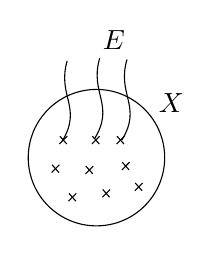
\begin{tikzpicture}[x=0.75pt,y=0.75pt,yscale=-1,xscale=1]
%uncomment if require: \path (0,300); %set diagram left start at 0, and has height of 300

%Flowchart: Connector [id:dp7499007648582767] 
\draw   (102,128.42) .. controls (102,110.26) and (116.72,95.55) .. (134.87,95.55) .. controls (153.02,95.55) and (167.74,110.26) .. (167.74,128.42) .. controls (167.74,146.57) and (153.02,161.29) .. (134.87,161.29) .. controls (116.72,161.29) and (102,146.57) .. (102,128.42) -- cycle ;
%Curve Lines [id:da20650999562395134] 
\draw    (118.28,120.59) .. controls (128.3,104.31) and (115.77,98.68) .. (120.78,81.77) ;
%Curve Lines [id:da9327641008081606] 
\draw    (133.93,119.34) .. controls (143.95,103.06) and (131.43,97.43) .. (136.43,80.52) ;
%Curve Lines [id:da6594075499360046] 
\draw    (147.08,119.97) .. controls (157.1,103.69) and (144.57,98.05) .. (149.58,81.15) ;
%Straight Lines [id:da13073640175251722] 
\draw    (117.25,118.09) -- (120.56,121.84) ;
%Straight Lines [id:da6620526994394944] 
\draw    (117.03,121.84) -- (120.78,118.09) ;

%Straight Lines [id:da8834541176981523] 
\draw    (132.9,118.09) -- (136.21,121.84) ;
%Straight Lines [id:da7510502290287235] 
\draw    (132.68,121.84) -- (136.43,118.09) ;

%Straight Lines [id:da44000068691517] 
\draw    (144.79,118.09) -- (148.11,121.84) ;
%Straight Lines [id:da8590400883175344] 
\draw    (144.57,121.84) -- (148.33,118.09) ;

%Straight Lines [id:da12268308784857629] 
\draw    (113.49,131.86) -- (116.81,135.62) ;
%Straight Lines [id:da22306917883937993] 
\draw    (113.27,135.62) -- (117.03,131.86) ;

%Straight Lines [id:da9728876585033619] 
\draw    (129.77,132.49) -- (133.08,136.24) ;
%Straight Lines [id:da23216656218706566] 
\draw    (129.55,136.24) -- (133.3,132.49) ;

%Straight Lines [id:da8478449055046726] 
\draw    (147.3,130.61) -- (150.61,134.37) ;
%Straight Lines [id:da7584484914378529] 
\draw    (147.08,134.37) -- (150.83,130.61) ;

%Straight Lines [id:da3145627797214947] 
\draw    (121.63,145.63) -- (124.94,149.39) ;
%Straight Lines [id:da696844406939886] 
\draw    (121.41,149.39) -- (125.17,145.63) ;

%Straight Lines [id:da4079053352483115] 
\draw    (137.91,143.76) -- (141.22,147.51) ;
%Straight Lines [id:da867418207840257] 
\draw    (137.69,147.51) -- (141.44,143.76) ;

%Straight Lines [id:da6401735618210065] 
\draw    (153.56,140.63) -- (156.87,144.38) ;
%Straight Lines [id:da7675951895008961] 
\draw    (153.34,144.38) -- (157.1,140.63) ;



% Text Node
\draw (163.62,96.13) node [anchor=north west][inner sep=0.75pt]   [align=left] {$X$};
% Text Node
\draw (136.7,66.07) node [anchor=north west][inner sep=0.75pt]   [align=left] {$E$};


\end{tikzpicture}
\end{figure}
\ei

Roughly speaking, 
observables are functions on fields, denoted as
$O(\sE)$ (or certain homology). For example, 
distributions are {\em linear observables}.

The new structures come from the following fact:
\begin{itemize}
\item Given an open subset $U\subset X$, we can talk about
\bea \operatorname{Obs}(U)= \text{observables supported in U}.\eea

\begin{eg}
$\sE=C^\infty(X),\ p\in X$. Consider 
\bea \cO_1: \sE \ra \bR,\eea
where $\cO_1(f)=f(p)^m, \ \forall f\in \sE$. $\cO_1$ is an observable supported in any open neighborhood of $p$.
\end{eg}

\item Let $\sE(U)=\Gamma(U,E)$. Then 
\bea
\operatorname{Obs}(U)=\text{functions on }  \sE(U).
\eea

\item The new structure is the \textbf{factorization product / operator product expansion (OPE)}. Given disjoint open subsets $U_i \subset V$, their disjoint union $\coprod_i U_i \subset V$, we have a map (factorization product):
\bea
\bigotimes_i \operatorname{Obs}(U_i)\mapsto \operatorname{Obs}(V).
\eea

\item Intuitively, if $\sE(U)$ is restricted to $\sE(U_i)$, then dually $O(\sE(U_i))\mapsto O(\sE(U))$.
Naively, we can {\em multiply} those {\em functions}, then we get
\bea
\bigotimes_i \operatorname{Obs}(U_i)\mapsto \operatorname{Obs}(V).
\eea
This, however, requires further {\em quantum corrections} in which fields in $U_i$'s may {\em talk} to each other.
\end{itemize}


\begin{eg}[Topological Quantum Mechanics]
In topological QFT, $\operatorname{Obs}(U)$ only depends on the topology of U.
Consider $\operatorname{dim} X=1$ and $\operatorname{Obs}(U)=A$ for a contractible open interval $U$. Now consider two open intervals $U_1$, $U_2$ on $X$ and embed them into a larger interval $V$.

\begin{figure}[!htpb]\centering
\tikzset{every picture/.style={line width=0.75pt}} %set default line width to 0.75pt        

\begin{tikzpicture}[x=0.75pt,y=0.75pt,yscale=-1,xscale=1]
%uncomment if require: \path (0,300); %set diagram left start at 0, and has height of 300

%Straight Lines [id:da6858804075591907] 
\draw    (370,108.54) -- (559.34,108.54) ;
%Straight Lines [id:da31596934900875695] 
\draw    (373.66,196.97) -- (563,196.97) ;
%Straight Lines [id:da32970695145900697] 
\draw    (469.7,128.89) -- (469.7,164.09) ;
\draw [shift={(469.7,166.09)}, rotate = 270] [color={rgb, 255:red, 0; green, 0; blue, 0 }  ][line width=0.75]    (10.93,-3.29) .. controls (6.95,-1.4) and (3.31,-0.3) .. (0,0) .. controls (3.31,0.3) and (6.95,1.4) .. (10.93,3.29)   ;

% Text Node
\draw (434.14,106.54) node   [align=left] {{\huge ( \ \ \ \ \ )}};
% Text Node
\draw (495.55,107.24) node   [align=left] {{\huge ( \ \ \ \ \ )}};
% Text Node
\draw (469.6,196.37) node   [align=left] {{\huge ( \ \ \ \ \ \ \ \ \ \ \ \ )}};
% Text Node
\draw (426.75,78.64) node [anchor=north west][inner sep=0.75pt]   [align=left] {$U_1$};
% Text Node
\draw (487.25,78.64) node [anchor=north west][inner sep=0.75pt]   [align=left] {$U_2$};
% Text Node
\draw (463.53,171.38) node [anchor=north west][inner sep=0.75pt]   [align=left] {$V$};

\end{tikzpicture}
\end{figure}

\noindent We have a topological quantum mechanics (QM) with maps
\bea
\operatorname{Obs}(U_1)\otimes \operatorname{Obs}(U_2) \mapsto \operatorname{Obs}(V)
\eea
or equivalently,
\bea
A \otimes A \mapsto A.
\eea
\end{eg}
\noindent We find an \textbf{associative algebra}!


\subsection*{Algebraic structure}
Consider two operators are placed at two different points on a line. When one operator approaches closely the other, the algebraic structure of the topology of the line comes from the homology group
\bea
H_{\bd} (\bR-\lcb 0\rcb)=H_0 (\bR-\lcb 0\rcb)= \bZ_{\text{Left}} \oplus \bZ_{\text{Right}}
\eea
which leads to left and right multiplications.

{\em Associativity} comes from further consistency:
\begin{figure}[!htpb]\centering
\tikzset{every picture/.style={line width=0.6pt}} %set default line width to 0.75pt        

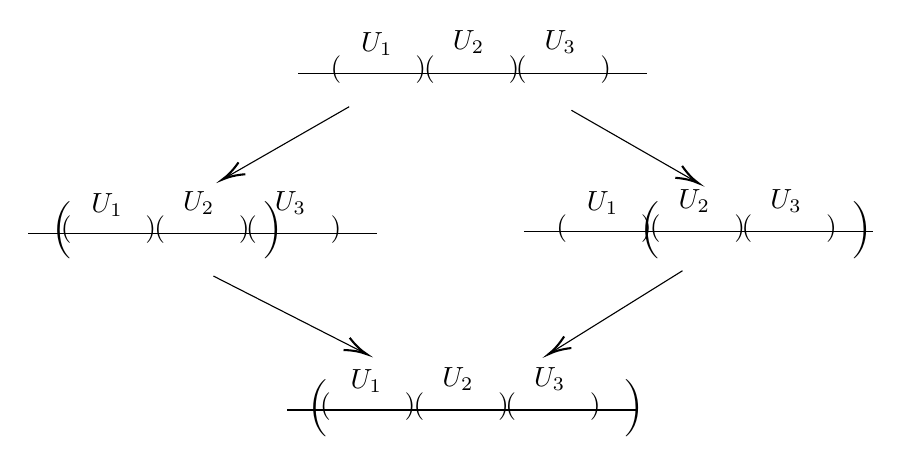
\begin{tikzpicture}[x=0.75pt,y=0.75pt,yscale=-1,xscale=1]
%uncomment if require: \path (0,300); %set diagram left start at 0, and has height of 300

%Straight Lines [id:da5543604292457156] 
\draw    (141,36.09) -- (309.24,36.09) ;
%Straight Lines [id:da4901487194099099] 
\draw    (11,113.41) -- (179.24,113.41) ;
%Straight Lines [id:da1721642744801426] 
\draw    (249.76,112.56) -- (418,112.56) ;
%Straight Lines [id:da22802491317770257] 
\draw    (135.9,198.38) -- (304.14,198.38) ;
%Straight Lines [id:da5450171031412938] 
\draw    (165.64,52.24) -- (106.2,86.36) ;
\draw [shift={(104.47,87.36)}, rotate = 330.14] [color={rgb, 255:red, 0; green, 0; blue, 0 }  ][line width=0.75]    (10.93,-3.29) .. controls (6.95,-1.4) and (3.31,-0.3) .. (0,0) .. controls (3.31,0.3) and (6.95,1.4) .. (10.93,3.29)   ;
%Straight Lines [id:da32782364610967507] 
\draw    (272.7,53.94) -- (332.15,88.06) ;
\draw [shift={(333.88,89.06)}, rotate = 209.86] [color={rgb, 255:red, 0; green, 0; blue, 0 }  ][line width=0.75]    (10.93,-3.29) .. controls (6.95,-1.4) and (3.31,-0.3) .. (0,0) .. controls (3.31,0.3) and (6.95,1.4) .. (10.93,3.29)   ;
%Straight Lines [id:da776515361469394] 
\draw    (100.22,133.81) -- (172.36,170.57) ;
\draw [shift={(174.14,171.48)}, rotate = 207] [color={rgb, 255:red, 0; green, 0; blue, 0 }  ][line width=0.75]    (10.93,-3.29) .. controls (6.95,-1.4) and (3.31,-0.3) .. (0,0) .. controls (3.31,0.3) and (6.95,1.4) .. (10.93,3.29)   ;
%Straight Lines [id:da4544384801263339] 
\draw    (326.23,131.26) -- (263.36,170.42) ;
\draw [shift={(261.66,171.48)}, rotate = 328.09] [color={rgb, 255:red, 0; green, 0; blue, 0 }  ][line width=0.75]    (10.93,-3.29) .. controls (6.95,-1.4) and (3.31,-0.3) .. (0,0) .. controls (3.31,0.3) and (6.95,1.4) .. (10.93,3.29)   ;

% Text Node
\draw (155.46,26.32) node [anchor=north west][inner sep=0.75pt]   [align=left] {( \ \ \ \ \ \ \ )};
% Text Node
\draw (200.5,26.32) node [anchor=north west][inner sep=0.75pt]   [align=left] {( \ \ \ \ \ \ \ )};
% Text Node
\draw (244.68,26.32) node [anchor=north west][inner sep=0.75pt]   [align=left] {( \ \ \ \ \ \ \ )};
% Text Node
\draw (170.16,15.27) node [anchor=north west][inner sep=0.75pt]   [align=left] {$U_1$};
% Text Node
\draw (214.35,14.42) node [anchor=north west][inner sep=0.75pt]   [align=left] {$U_2$};
% Text Node
\draw (258.53,14.42) node [anchor=north west][inner sep=0.75pt]   [align=left] {$U_3$};
% Text Node
\draw (25.46,103.64) node [anchor=north west][inner sep=0.75pt]   [align=left] {( \ \ \ \ \ \ \ )};
% Text Node
\draw (70.49,103.64) node [anchor=north west][inner sep=0.75pt]   [align=left] {( \ \ \ \ \ \ \ )};
% Text Node
\draw (114.68,103.64) node [anchor=north west][inner sep=0.75pt]   [align=left] {( \ \ \ \ \ \ \ )};
% Text Node
\draw (40.16,92.59) node [anchor=north west][inner sep=0.75pt]   [align=left] {$U_1$};
% Text Node
\draw (84.34,91.74) node [anchor=north west][inner sep=0.75pt]   [align=left] {$U_2$};
% Text Node
\draw (128.53,91.74) node [anchor=north west][inner sep=0.75pt]   [align=left] {$U_3$};
% Text Node
\draw (264.22,102.79) node [anchor=north west][inner sep=0.75pt]   [align=left] {( \ \ \ \ \ \ \ )};
% Text Node
\draw (309.26,102.79) node [anchor=north west][inner sep=0.75pt]   [align=left] {( \ \ \ \ \ \ \ )};
% Text Node
\draw (353.44,102.79) node [anchor=north west][inner sep=0.75pt]   [align=left] {( \ \ \ \ \ \ \ )};
% Text Node
\draw (278.92,91.74) node [anchor=north west][inner sep=0.75pt]   [align=left] {$U_1$};
% Text Node
\draw (323.11,90.89) node [anchor=north west][inner sep=0.75pt]   [align=left] {$U_2$};
% Text Node
\draw (367.29,90.89) node [anchor=north west][inner sep=0.75pt]   [align=left] {$U_3$};
% Text Node
\draw (150.37,188.61) node [anchor=north west][inner sep=0.75pt]   [align=left] {( \ \ \ \ \ \ \ )};
% Text Node
\draw (195.4,188.61) node [anchor=north west][inner sep=0.75pt]   [align=left] {( \ \ \ \ \ \ \ )};
% Text Node
\draw (239.58,188.61) node [anchor=north west][inner sep=0.75pt]   [align=left] {( \ \ \ \ \ \ \ )};
% Text Node
\draw (165.06,177.56) node [anchor=north west][inner sep=0.75pt]   [align=left] {$U_1$};
% Text Node
\draw (209.25,176.71) node [anchor=north west][inner sep=0.75pt]   [align=left] {$U_2$};
% Text Node
\draw (253.43,176.71) node [anchor=north west][inner sep=0.75pt]   [align=left] {$U_3$};
% Text Node
\draw (21.2,96.76) node [anchor=north west][inner sep=0.75pt]   [align=left] {{\huge ( \ \ \ \ \ \ \ \ \ \ )}};
% Text Node
\draw (304.9,96.76) node [anchor=north west][inner sep=0.75pt]   [align=left] {{\huge ( \ \ \ \ \ \ \ \ \ \ )}};
% Text Node
\draw (144.88,182.24) node [anchor=north west][inner sep=0.75pt]   [align=left] {{\huge ( \ \ \ \ \ \ \ \ \ \ \ \ \ \ \ \ )}};
\end{tikzpicture}
\end{figure}
\bea
\RA (a\cdot b)\cdot c= a\cdot (b\cdot c).
\eea

\begin{eg}[Chiral QFT] $\operatorname{dim }X=2$ (a plane). 
\begin{figure}[!htpb]\centering


\tikzset{every picture/.style={line width=0.75pt}} %set default line width to 0.75pt        

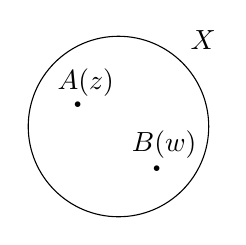
\begin{tikzpicture}[x=0.75pt,y=0.75pt,yscale=-1,xscale=1]
%uncomment if require: \path (0,300); %set diagram left start at 0, and has height of 300

%Shape: Ellipse [id:dp8384382557053032] 
\draw   (66.98,120.35) .. controls (66.98,96.34) and (86.45,76.87) .. (110.46,76.87) .. controls (134.48,76.87) and (153.94,96.34) .. (153.94,120.35) .. controls (153.94,144.37) and (134.48,163.83) .. (110.46,163.83) .. controls (86.45,163.83) and (66.98,144.37) .. (66.98,120.35) -- cycle ;

% Text Node
\draw (79.83,91.45) node [anchor=north west][inner sep=0.75pt]   [align=left] {$A(z)$};
% Text Node
\draw (115.66,121.35) node [anchor=north west][inner sep=0.75pt]   [align=left] {$B(w)$};
% Text Node
\draw (85.82,107.186) node [anchor=north west][inner sep=0.75pt]   [align=left] {{\Huge .}};
% Text Node
\draw (123.79,137.86) node [anchor=north west][inner sep=0.75pt]   [align=left] {{\Huge .}};
% Text Node
\draw (144,73) node [anchor=north west][inner sep=0.75pt]   [align=left] {$X$};
\end{tikzpicture}

\end{figure}

\noindent In holomorphic coordinates, when an operator approach (wind around) the other on $X$, the winding number can be kept track in terms of their Laurent modes:
\bea 
A(z)B(w)=\sum_{m\in \bZ}\frac{\lb A_{(m)}B\rb (w)}{(z-w)^{m+1}}.
\eea
We find $\infty$-many ``product'' (binary operation) $\lcb A_{(m)}B \rcb$. Observable algebras then give rise to \textbf{vertex algebras}.
\end{eg}

These observable algebras are developed in the works of:
\begin{itemize}
    \item Beilinson-Drinfeld
    \begin{itemize}
        \item developed factorization algebra to formulate two-dimensional chiral conformal field theory (CFT)
        \item introduced the notion of {\em chiral homology} (generalize {\em Hodge homology} in one dimension)
    \end{itemize}
    \item Costello-Gwilliam
    \begin{itemize}
        \item constructed factorization algebras from perturbative renormalization theory, in the \textbf{Batalin-Vilkovisky (BV) formalism} (generalize BRST formalism in gauge theory).
    \end{itemize}
\end{itemize}

%\begin{rem} The geometrical study of QFT are related to index theory: 1-dim. (Atiyah-Singer index theory), 2-dim. (chiral index theory on loop space). (see later) \end{rem}

\subsection*{BV formalism and homological integration}
    \bea \int \ =\ \text{homology}\eea
\begin{itemize}
    \item \underline{Calculus revisited}\\
    Let $M$ be a compact oriented manifold of $\operatorname{dim} M=n$. Many constructions of integration on manifolds can be understood from de Rham complex
    $\lb \Omega^\bd(M), d\rb$. Consider the integration map 
    \bea
    \int_M: \Omega^\bd(M) \ra \bR,\qquad
    \alpha\in \Omega^n(M) \mapsto \int_M \alpha. \eea
    Observe that the $n$-th de Rham cohomology group
    $H^n_{dR}(M) =\bR$. This implies that 
    \bea
    \int_M \ = \ H^n_{dR}. \eea
    The integration map is now
    \bea
    \Omega^n(M) \ra H^n_{dR}(M),\qquad
    \alpha \mapsto [\alpha].
    \eea
    This means that we can learn calculus by the algebraic structure on de Rham complex, even we do not know anything about measure theory. However, there is a problem of understanding $H^n_{dR}(M)$ when $n\ra\infty$ as in QFT.
    
    \item \underline{BV approach}\\
    Define \textbf{polyvector fields}
    \bea 
    \operatorname{PV}^\bd(M) =\bigoplus_k \operatorname{PV}^k(M)\coloneqq \bigoplus_k \Gamma \lb M,\ \bigw^k TM\rb.
     \eea
    Let $\Omega$ be a fixed volume form on $M$. We can naturally identify
    \bea
    \operatorname{PV}^k(M) \lra \Omega ^{n-k}(M),\qquad
    \mu\in \operatorname{PV}^k(M) \lra \mu \lrcorner \Omega.
    \eea
    Locally, if $\Omega=e^\varphi dx^1\wedge \cdots \wedge dx^n$, $\mu=\mu^{i_1\cdots i_k} \partial_{i_1}\wedge \cdots \wedge \partial_{i_k}$, then
    \bea \mu \lrcorner\Omega= \sum \pm \mu^{i_1\cdots i_k} e^\varphi dx^1 \wedge \cdots \wedge \widehat{dx^{i_1}}\wedge \cdots \wedge\widehat{dx^{i_k}} \wedge \cdots \wedge dx^n. \eea
    
    The identification above leads to 
    \begin{figure}[!htpb]\centering
\tikzset{every picture/.style={line width=0.75pt}} %set default line width to 0.75pt        

\begin{tikzpicture}[x=0.75pt,y=0.75pt,yscale=-1,xscale=1]
%uncomment if require: \path (0,300); %set diagram left start at 0, and has height of 300

%Straight Lines [id:da7418770892542212] 
\draw    (77,75) -- (108.33,75) ;
\draw [shift={(110.33,75)}, rotate = 180] [color={rgb, 255:red, 0; green, 0; blue, 0 }  ][line width=0.75]    (10.93,-3.29) .. controls (6.95,-1.4) and (3.31,-0.3) .. (0,0) .. controls (3.31,0.3) and (6.95,1.4) .. (10.93,3.29)   ;
%Straight Lines [id:da7789911226523776] 
\draw    (150,75) -- (181.33,75) ;
\draw [shift={(183.33,75)}, rotate = 180] [color={rgb, 255:red, 0; green, 0; blue, 0 }  ][line width=0.75]    (10.93,-3.29) .. controls (6.95,-1.4) and (3.31,-0.3) .. (0,0) .. controls (3.31,0.3) and (6.95,1.4) .. (10.93,3.29)   ;
%Straight Lines [id:da8825213733946038] 
\draw    (212,74) -- (243.33,74) ;
\draw [shift={(245.33,74)}, rotate = 180] [color={rgb, 255:red, 0; green, 0; blue, 0 }  ][line width=0.75]    (10.93,-3.29) .. controls (6.95,-1.4) and (3.31,-0.3) .. (0,0) .. controls (3.31,0.3) and (6.95,1.4) .. (10.93,3.29)   ;
%Straight Lines [id:da6853513626542171] 
\draw    (74,124) -- (105.33,124) ;
\draw [shift={(107.33,124)}, rotate = 180] [color={rgb, 255:red, 0; green, 0; blue, 0 }  ][line width=0.75]    (10.93,-3.29) .. controls (6.95,-1.4) and (3.31,-0.3) .. (0,0) .. controls (3.31,0.3) and (6.95,1.4) .. (10.93,3.29)   ;
%Straight Lines [id:da40948388226369414] 
\draw    (155,124) -- (186.33,124) ;
\draw [shift={(188.33,124)}, rotate = 180] [color={rgb, 255:red, 0; green, 0; blue, 0 }  ][line width=0.75]    (10.93,-3.29) .. controls (6.95,-1.4) and (3.31,-0.3) .. (0,0) .. controls (3.31,0.3) and (6.95,1.4) .. (10.93,3.29)   ;
%Straight Lines [id:da4080909117329181] 
\draw    (207,124) -- (238.33,124) ;
\draw [shift={(240.33,124)}, rotate = 180] [color={rgb, 255:red, 0; green, 0; blue, 0 }  ][line width=0.75]    (10.93,-3.29) .. controls (6.95,-1.4) and (3.31,-0.3) .. (0,0) .. controls (3.31,0.3) and (6.95,1.4) .. (10.93,3.29)   ;

% Text Node
\draw (83,58) node [anchor=north west][inner sep=0.75pt]   [align=left] {$d$};
% Text Node
\draw (191,63) node [anchor=north west][inner sep=0.75pt]   [align=left] {$\cdots$};
% Text Node
\draw (157,58) node [anchor=north west][inner sep=0.75pt]   [align=left] {$d$};
% Text Node
\draw (219,57) node [anchor=north west][inner sep=0.75pt]   [align=left] {$d$};
% Text Node
\draw (47,66.4) node [anchor=north west][inner sep=0.75pt]    {$\Omega ^{0}$};
% Text Node
\draw (121,65.4) node [anchor=north west][inner sep=0.75pt]    {$\Omega ^{1}$};
% Text Node
\draw (249,64.4) node [anchor=north west][inner sep=0.75pt]    {$\Omega ^{n}$};
% Text Node
\draw (190,112) node [anchor=north west][inner sep=0.75pt]   [align=left] {$\cdots$};
% Text Node
\draw (41,115.4) node [anchor=north west][inner sep=0.75pt]    {$PV^{n}$};
% Text Node
\draw (81,103.4) node [anchor=north west][inner sep=0.75pt]    {$\Delta $};
% Text Node
\draw (163,105.4) node [anchor=north west][inner sep=0.75pt]    {$\Delta $};
% Text Node
\draw (216,104.4) node [anchor=north west][inner sep=0.75pt]    {$\Delta $};
% Text Node
\draw (109,113.4) node [anchor=north west][inner sep=0.75pt]    {$PV^{n-1}$};
% Text Node
\draw (241,113.4) node [anchor=north west][inner sep=0.75pt]    {$PV^{0}$};
% Text Node
\draw (61.81,87.57) node [anchor=north west][inner sep=0.75pt]  [rotate=-88.54,xslant=0.03]  {$\cong $};
% Text Node
\draw (133.81,87.57) node [anchor=north west][inner sep=0.75pt]  [rotate=-88.54,xslant=0.03]  {$\cong $};
% Text Node
\draw (263.81,87.57) node [anchor=north west][inner sep=0.75pt]  [rotate=-88.54,xslant=0.03]  {$\cong $};
% Text Node
\draw (286.14,46.01) node [anchor=north west][inner sep=0.75pt]  [font=\Large,rotate=-28.13]  {$\xrightarrow{\ \ \int \ \ }$};
% Text Node
\draw (269.44,119.51) node [anchor=north west][inner sep=0.75pt]  [font=\Large,rotate=-332.79]  {$\xrightarrow[   \ \int_{\text{BV}}\ ]{}$};
% Text Node
\draw (318,86.4) node [anchor=north west][inner sep=0.75pt]    {$\bR$};
\end{tikzpicture}
\end{figure}

where
$\Delta: \operatorname{PV}^k \ra \operatorname{PV}^{k-1}$ is a divergence operator with respect to $\Omega$. $\Delta$ is called the \textbf{BV operator}.
For example, 
$\Delta: \operatorname{PV}^1=\operatorname{Vect}(M) \ra \operatorname{PV}^0=C^\infty(M)$ is the usual divergence.
$\int_{\operatorname{BV}}$ is the \textbf{BV integration}, which is a map:
\bea \int_{\operatorname{BV}}: \operatorname{PV}^0 \ra \bR,\qquad 
f \mapsto \int f\Omega.
\eea

Homologically $\int_{\operatorname{BV}}$ can be identified with $H^0_{\operatorname{BV}}$.
Here ``$\operatorname{dim} (M)$'' does not appear. The problem of integration is transferred to construct $\Delta$, which has a convenient formulation at least in perturbative QFT.
In $\infty$-dimensions (as in QFT), renormalization helps to construct $\Delta$ which leads to \textbf{homological integration}.

\item \underline{Explicit form of $\Delta$}\\
Locally in $U$, let $\lcb x_i\rcb_{i=1}^n$ be local coordinates, the volume form be $\Omega=e^{f(x)}dx^1\wedge \cdots \wedge dx^n$. Introduce the vector fields $\partial_i=\frac{\partial}{\partial x_i}$, then the polyvector field is \bea \operatorname{PV}(U)=C^\infty(U) [\partial_1, \cdots, \partial_n],\eea
where $\partial_i$'s are anticommuting: $\partial_i \partial_j =- \partial_j \partial_i$. 
Let us write $\theta_i=\partial_i$ (\textit{note}: this is a vector field, NOT an differential operator), then a local section $\mu\in \operatorname{PV}(X)$ can be written as a function of $x^i$, $\theta_i$:
\bea
\mu=\mu (x^i, \theta_i)
\eea
with $x^ix^j=x^j x^i$ and $\theta_i \theta_j =- \theta_j \theta_i$.
Let $\frac{\partial}{\partial x^i}$ be the derivative with respect to $x^i$  and $\frac{\partial}{\partial \theta_i}$ be the derivative with respect to $\theta_i$ (from the left). Then the BV operator is given locally by 
\bea
\Delta = \sum_i \frac{\partial}{\partial x^i} \frac{\partial}{\partial \theta_i}
+\sum_i (\partial_i f) \frac{\partial}{\partial \theta_i}
\eea
which looks like a second order operator (it is easy to check that $\Delta^2=0$). This is in contrast with de Rham differential $d$, which is a first order differential
operator. Note that the first term looks like a Laplacian, but it is NOT. $\theta_i$ is an odd variable. Hence, $\Delta$ is sometimes called an {\em odd Laplacian}.

\begin{eg}[$\frac{\partial}{\partial \theta_i}$ operator]
\bea\frac{\partial}{\partial \theta_1}(\theta_1\theta_2)=\theta_2,\\
\frac{\partial}{\partial \theta_1}(\theta_2\theta_1)=- \frac{\partial}{\partial \theta_1}(\theta_1\theta_2)=-\theta_2.
\eea
\end{eg}

\begin{eg}[Singularity theory]
Consider the $n$-th dimensional complex space $\bC^n$. Let $f: \bC^n\ra \bC$ be a polynomial in $n$ variables with an isolated critical pint at 0:
\bea \operatorname{Crit}(f)=\lcb 0\rcb.\eea
We consider holomorphic/polynomial polyvector fields
\bea \cA =\bC[z^i, \theta_i], \quad
\theta_i \theta_j =- \theta_j \theta_i.\eea
Let the BV operator be
\bea \Delta=\hbar \sum_{i=1}^n \frac{\partial}{\partial z^i} \frac{\partial}{\partial \theta_i}
+\sum_i (\partial_i f) \frac{\partial}{\partial \theta_i}. \eea
\begin{itemize}
    \item The space of quantum observables $\operatorname{Obs}^q=H^\bd (\cA[[\hbar]],\Delta)$ is isomorphic to a formal completion of the Brieskorn lattice.
    \item 
    The quantum observable (or Brieskorn lattice) plays an important role of Hodge filtration (which is related to $\hbar$-filtration) in singularity theory.
    \item The BV-integration models the oscillatory integral 
    \bea\lan \cO\ran=\int_{\mathscr{L}} d^n z\ \cO e^{f/\hbar},\eea where $\mathscr{L}$ is a Lefschetz thimble.
\end{itemize}
\end{eg}
\end{itemize}

\noindent{\em Reference}: \cite{Li:2017exk}

\section{Perturbative theory and Feynman diagram}
Understanding the path integral $\int e^{-S/\hbar}$ on the full space of fields is difficult. We can, however, have a well understanding of the behavior of a theory around the critical points of the action functional $S$. We will work on the asymptotic $\hbar$-expansion around the minima of $S$. This perturbative theory has a very nice combinatorial expression --- Feynman diagrams, which also has physical interpretations. We present this result via the {\em BV idea}. This idea is different from the usual approach to Feynman diagrams, but it has an advantage that its homological interpretation can be used in formulating index theory.

As discussed in the \nameref{sec:intro}, given a volume form
\bea \Omega=e^{f(x)} dx^1\wedge \cdots \wedge dx^n,\eea
we can consider the integration map 
\bea
\int: \ \cA
\ra \bR,\eea
where $\cA$ is a function on $\lcb x^i,\theta_i\rcb$, where $\theta_i$'s are anticommuting variables, $\theta_i \theta_j =- \theta_j \theta_i$. 
If we integrate over $\bR^n$, $\int_{\bR^n}$ picks only the components without $\theta_i$'s (i.e. the $\operatorname{PV}^0$-part) and
\bea \int_{\bR^n}: f(x)\mapsto \int_{\bR^n} f(x)\Omega.\eea
This integration is defined on BV homology ($\Delta$-homology), where 
$\Delta: \cA \ra \cA$ is the BV-operator given by
\bea \Delta= \sum_{i=1}^n \frac{\partial}{\partial x^i} \frac{\partial}{\partial \theta_i}
+\sum_i (\partial_i f) \frac{\partial}{\partial \theta_i}. \eea

\begin{eg} An integral over a $\Delta$-exact term vanishes, i.e.
\bea\int_{\bR^n}\Delta(\varphi^i(x)\theta_i)\Omega=0.\eea
This looks like Stokes' theorem.
Explicitly,
\bea\int_{\bR^n} d^n x \lb \sum_i \partial_i\varphi^i+\sum_i \varphi^i\partial_i f\rb e^f =0. \eea
It vanishes after the integration by part is performed.
\end{eg}

\subsection*{Gaussian integral}
Consider the simplest example: a one-dimensional real space $\bR$ and a Gaussian-type volume form
\bea \Omega= \frac{1}{\sqrt{2\pi}} e^{-\hf x^2} dx.\eea
We study the integration map on polynomial functions:
\bea\int: \ \bR[x]\ra \bC,\qquad g(x)\mapsto\int_\bR g(x)\Omega \eea
or more generally,
\bea\int: \ \bR[x,\theta]\ra \bC,\qquad g(x)+h(x)\theta \mapsto\int_\bR g(x)\Omega \qquad (\theta^2=0).\eea
The BV operator reads
\bea
\Delta = \frac{\partial}{\partial x} \frac{\partial}{\partial \theta}
-x \frac{\partial}{\partial \theta}.
\eea
Here $f= -\hf x^2$. Given any polynomial $g(x)\in \bR[x]$, we have
\bea \Delta g=0\eea
since $g$ has no $\theta$'s. Let $[g]_{\Delta}$ denote the \textbf{$\Delta$-cohomology classes}, in which
\bea
\lsb g_1\rsb_{\Delta}=\lsb g_2\rsb_{\Delta}\ \LRA \ g_1-g_2=\Delta \eta \ \text{for some } \eta\in \bR[x,\theta].
\eea
Then $\int$ is well-defined on $\Delta$-cohomology classes:
\bea \int g_1\Omega= \int g_2\Omega \quad  \text{if } 
\lsb g_1\rsb_{\Delta}=\lsb g_2\rsb_{\Delta}.\eea
We also have the normalization of the Gaussian integral:
\bea \int 1\ \Omega =1.\eea

\begin{eg}
\bea \Delta \lb x^{m-1}\theta\rb &=
\lb\frac{\partial}{\partial x} \frac{\partial}{\partial \theta}
-x \frac{\partial}{\partial \theta}\rb \lb x^{m-1}\theta\rb
=(m-1)x^{m-2} -x^m\\
\RA \lsb x^m\rsb_{\Delta} &= (m-1) \lsb x^{m-2}\rsb_{\Delta}\\
\RA \lsb x^{2k}\rsb_{\Delta} &= (2k-1)!! \lsb 1\rsb_{\Delta}\\
\RA \int_{\bR} x^{2k}\Omega &= 
(2k-1)!! \int_{\bR}\Omega= 
(2k-1)!!.\eea
\end{eg}

To organize the data, consider the following operator
\bea \cU=e^{\hf \frac{\partial}{\partial x} \frac{\partial}{\partial x}}: \bR\lsb x,\theta\rsb \ra \bR\lsb x,\theta\rsb.\eea
Explicitly, $\cU\lb g(x)+h(x)\theta\rb= 
\lb \cU g(x)\rb+ \lb \cU h(x)\rb \theta,$ where $\cU$ acts on polynomials via Taylor expansion
\bea \cU=\sum_{k=0}^\infty \frac{1}{k!} \lb \hf \frac{\partial}{\partial x} \frac{\partial}{\partial x} \rb^k \eea
which is well-defined on $\bR[x]$.

\begin{lem}
The BV operator is given by
\bea \Delta= \cU^{-1}\lb -x\frac{\partial}{\partial\theta}\rb \cU\eea
i.e. $\Delta$ is conjugate to the simple operation $-x\frac{\partial}{\partial\theta}$ via the operator $\cU$.
\end{lem}
\noindent The proof to this lemma is left as an exercise to the reader.

As a result, we find a {\em cochain isomorphism} of complexes
\bea \cU: \lb \bR\lsb x,\theta\rsb,\Delta\rb \ra \lb \bR\lsb x,\theta\rsb,-x\frac{\partial}{\partial\theta}\rb, \qquad 1\mapsto 1.
\eea
Cochain map means that
\bea \cU \circ \Delta(\varphi)= \lb -x\frac{\partial}{\partial\theta}\rb\circ \cU(\varphi) \eea
i.e. $\cU$ intertwines $\Delta$ with $-x\frac{\partial}{\partial\theta}$.

Observe that
\bea
H^\bd \lb \bR\lsb x,\theta \rsb, 
-x\frac{\partial}{\partial\theta}\rb
=H^0 \lb \bR\lsb x,\theta \rsb, 
-x\frac{\partial}{\partial\theta}\rb=\bR.
\eea
Let $\lsb -\rsb_{-x\partial_\theta}$ represent the $\lb -x\frac{\partial}{\partial\theta}\rb$-cohomology classes. Then for any $m>0$, $x^m=\lb -x\frac{\partial}{\partial\theta}\rb \lb-x^{m-1}\theta\rb$. Hence,
\bea \lsb h(x)\rsb_{-x\partial_\theta}= \lsb h(0)\rsb_{-x\partial_\theta}\eea
for an arbitrary polynomial $h(x)$. All higher power terms beyond the constant terms are exact; hence they vanish.
Now for any $g(x)\in \bR\lsb x\rsb$,

\begin{figure}[!htpb]\centering
\tikzset{every picture/.style={line width=0.75pt}} %set default line width to 0.75pt        
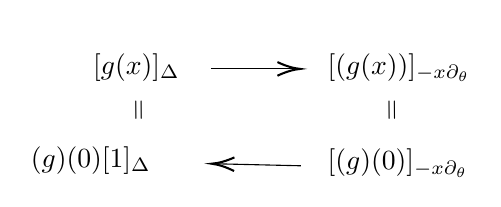
\begin{tikzpicture}[x=0.75pt,y=0.75pt,yscale=-1,xscale=1]
%uncomment if require: \path (0,300); %set diagram left start at 0, and has height of 300

%Straight Lines [id:da7851604577852263] 
\draw    (129,41) -- (170,41) ;
\draw [shift={(172,41)}, rotate = 180] [color={rgb, 255:red, 0; green, 0; blue, 0 }  ][line width=0.75]    (10.93,-3.29) .. controls (6.95,-1.4) and (3.31,-0.3) .. (0,0) .. controls (3.31,0.3) and (6.95,1.4) .. (10.93,3.29)   ;
%Straight Lines [id:da2533793961040385] 
\draw    (172.33,87.67) -- (131.33,86.71) ;
\draw [shift={(129.33,86.67)}, rotate = 1.33] [color={rgb, 255:red, 0; green, 0; blue, 0 }  ][line width=0.75]    (10.93,-3.29) .. controls (6.95,-1.4) and (3.31,-0.3) .. (0,0) .. controls (3.31,0.3) and (6.95,1.4) .. (10.93,3.29)   ;

% Text Node
\draw (71,32.4) node [anchor=north west][inner sep=0.75pt]    {$[ g( x)]_{\Delta }$};
% Text Node
\draw (141,21.4) node [anchor=north west][inner sep=0.75pt]    {$\cU$};
% Text Node
\draw (184,32.4) node [anchor=north west][inner sep=0.75pt]    {$[ \cU( g( x))]_{-x\partial _{\theta }}$};
% Text Node
\draw (97.01,54.44) node [anchor=north west][inner sep=0.75pt]  [rotate=-89.57]  {$=$};
% Text Node
\draw (219.01,54.44) node [anchor=north west][inner sep=0.75pt]  [rotate=-89.57]  {$=$};
% Text Node
\draw (184,78.4) node [anchor=north west][inner sep=0.75pt]    {$[ \cU( g)( 0)]_{-x\partial _{\theta }}$};
% Text Node
\draw (41,77.4) node [anchor=north west][inner sep=0.75pt]    {$\cU( g)( 0)[ 1]_{\Delta }$};
\end{tikzpicture}
\end{figure}
\noindent we find 
\bea \lsb g(x)\rsb_{\Delta}= \cU(g)(0)\lsb 1\rsb_{\Delta}.\eea
In other words, 
\bea
\int_{\bR} g(x)\Omega\ =\left. e^{\hf \partial_x^2} g(x)\right|_{x=0} \int_{\bR} 1\Omega \ =\left. e^{\hf \partial_x^2} g(x)\right|_{x=0}.
\eea

In general, we can introduce a new parameter $a$. 
\begin{prop}\label{prop1}
\bea \int_\bR g(x+a)\Omega = e^{\hf \partial_a^2}g(a),\quad  \forall g\in \bR[x].\eea
\end{prop}
\noindent The shift by $a$ has the interpretation of effective fields as well as background fields, which is related to homological perturbation. The upshot now is that the integration $\int \lb\cdots \rb \Omega$ is fully described by the operator $\cU$.

Now we consider a toy model:
\bea
\int_\bR \frac{dx}{\sqrt{2\pi\hbar}}\ e^{\lb -\hf x^2+\frac{\lambda}{3!}x^3\rb /\hbar}, \quad \lambda\in\bR.
\eea
This integral is in fact divergent since $x^3$ blows up quickly at $\infty$. There are two ways out of this problem. 
\bi[(1)]
    \item Treat $x$ as a complex variable and change the integration cycle from $\bR$ (i.e. $\Re(x)$) to some integration cycles $\Gamma_i\in \bC$:
    \bea \int_{\Gamma_i}\frac{dx}{\sqrt{2\pi\hbar}}\ e^{\lb -\hf x^2+\frac{\lambda}{3!}x^3\rb /\hbar}, \quad x\in\bC,\ \lambda\in\bR.\eea
    
    \bea
\tikzset{every picture/.style={line width=0.75pt}} %set default line width to 0.75pt        
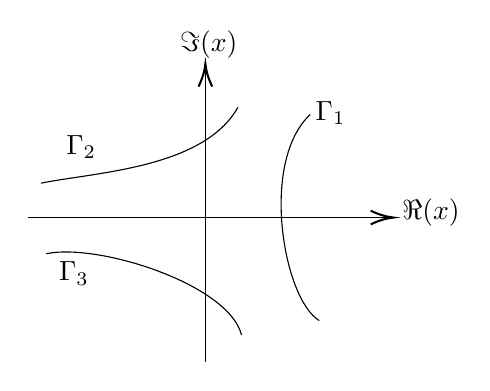
\begin{tikzpicture}[x=0.75pt,y=0.75pt,yscale=-1,xscale=1]
%uncomment if require: \path (0,300); %set diagram left start at 0, and has height of 300

%Straight Lines [id:da772733815126962] 
\draw    (127.35,195) -- (127.35,53.29) ;
\draw [shift={(127.35,51.29)}, rotate = 90] [color={rgb, 255:red, 0; green, 0; blue, 0 }  ][line width=0.75]    (10.93,-3.29) .. controls (6.95,-1.4) and (3.31,-0.3) .. (0,0) .. controls (3.31,0.3) and (6.95,1.4) .. (10.93,3.29)   ;
%Straight Lines [id:da03837733772961949] 
\draw    (42,125.32) -- (215.94,125.32) ;
\draw [shift={(217.94,125.32)}, rotate = 180] [color={rgb, 255:red, 0; green, 0; blue, 0 }  ][line width=0.75]    (10.93,-3.29) .. controls (6.95,-1.4) and (3.31,-0.3) .. (0,0) .. controls (3.31,0.3) and (6.95,1.4) .. (10.93,3.29)   ;
%Curve Lines [id:da1873702300348834] 
\draw    (177.87,75.68) .. controls (153.48,98.32) and (164.81,164.52) .. (182.23,174.97) ;
%Curve Lines [id:da9465928462718054] 
\draw    (143.03,72.19) .. controls (126.48,101.81) and (73.35,103.55) .. (48.1,108.77) ;
%Curve Lines [id:da48991182789985976] 
\draw    (144.77,181.94) .. controls (138.68,157.55) and (75.97,137.52) .. (50.71,142.74) ;

% Text Node
\draw (179.26,67.95) node [anchor=north west][inner sep=0.75pt]    {$\Gamma _{1}$};
% Text Node
\draw (59.06,84.5) node [anchor=north west][inner sep=0.75pt]    {$\Gamma _{2}$};
% Text Node
\draw (55.58,145.46) node [anchor=north west][inner sep=0.75pt]    {$\Gamma _{3}$};
% Text Node
\draw (220.97,115.11) node [anchor=north west][inner sep=0.75pt]    {$\Re ( x)$};
% Text Node
\draw (113.9,34.11) node [anchor=north west][inner sep=0.75pt]    {$\Im ( x)$};
\end{tikzpicture}
\eea
    This becomes the Airy integral. 
    
    \item Treat the integral as an asymptotic series in $\lambda$ via
    \bea e^{\frac{\lambda}{3!\hbar}x^3}= \sum_{n\geq 0} \frac{\lb \frac{\lambda}{3!\hbar}x^3\rb^n}{n!}.\eea
\ei

Let's focus on method (2). This is known as the {\em perturbative theory}. We will also add the background parameter $a$ in our integral.
\bea \int_\bR \frac{dx}{\sqrt{2\pi\hbar}}\ e^{\lb -\hf x^2+\frac{\lambda}{3!}(x+a)^3\rb /\hbar}
\ =\ e^{\frac{\hbar}{2}\partial_a^2} e^{\frac{\lambda}{3!\hbar}a^3}
\ =\ \sum_{k,m\geq 0} 
\frac{\lb \frac{\hbar}{2}\partial_a^2\rb^k}{k!}
\frac{\lb  \frac{\lambda}{3!\hbar}a^3\rb^m}{m!}.
\eea
We have used the fact (Proposition \ref{prop1}) that the integration $\int_\bR \frac{dx}{\sqrt{2\pi\hbar}} g(x+a) e^{-\frac{1}{2\hbar} x^2}$ is described by the operator $e^{\frac{\hbar}{2} \partial_a^2}g(a)$. This infinite sum can be organized into graphs (or Feynman diagrams). Here are some examples.
\begin{itemize}
    \item one term in $\lb \frac{\hbar}{2}\partial_a^2\rb^2
    \lb \frac{\lambda}{3!\hbar}a^3\rb^2$ has
    \bea
    \begin{fmffile}{fd1}
    \begin{tabular}{c}
        \begin{fmfgraph*}(100,60)
                \fmfleft{i}
                \fmfright{o}
                \fmf{plain,tension=4}{i,v1}
                \fmf{plain,tension=4}{v2,o}
                \fmf{plain,left,label=$\frac{\hbar}{2}\partial_a\otimes\partial_a$,label.side=left,tension=1}{v1,v2,v1}
                \fmfv{label=$\frac{\lambda}{\hbar}$,label.angle=120,decor.shape=circle,decor.filled=full,decor.size=2thick}{v1}
                \fmfv{label=$\frac{\lambda}{\hbar}$,label.angle=60,decor.shape=circle,decor.filled=full,decor.size=2thick}{v2}
                \fmflabel{$a$}{i}
                \fmflabel{$a$}{o}
        \end{fmfgraph*}
        \end{tabular}
    \end{fmffile}
    ~~~~~~~~ \sim\ \lambda^2 a^2.
    \eea
    
    \item one term in $\lb \frac{\hbar}{2}\partial_a^2\rb
    \lb \frac{\lambda}{3!\hbar}a^3\rb^2$ has
    \bea
    \begin{fmffile}{fd2}
    \begin{tabular}{c}
        \begin{fmfgraph*}(100,60)
                \fmfleft{i1,i2}
                \fmfright{o1,o2}
                \fmf{plain,tension=.5}{i1,v1}
                \fmf{plain,tension=.5}{i2,v1}
                \fmf{plain,tension=.5}{v2,o1}
                \fmf{plain,tension=.5}{v2,o2}
                \fmf{plain,label=$\hbar \partial_a\otimes\partial_a$,label.side=left,tension=.4}{v1,v2}
                \fmfv{label=$\frac{\lambda}{\hbar}$,label.angle=180,decor.shape=circle,decor.filled=full,decor.size=2thick}{v1}
                \fmfv{label=$\frac{\lambda}{\hbar}$,label.angle=0,decor.shape=circle,decor.filled=full,decor.size=2thick}{v2}
                \fmflabel{$a$}{i1}
                \fmflabel{$a$}{i2}
                \fmflabel{$a$}{o1}
                \fmflabel{$a$}{o2}
        \end{fmfgraph*}
        \end{tabular}
    \end{fmffile}
    ~~~~~~~~ \sim\ \frac{\lambda^2}{\hbar}a^4.
    \eea
\end{itemize}

In general, given a graph $\Gamma$, let
\bea
D &=\text{number of external edges},\\
E &=\text{number of internal edges},\\
V &=\text{number of vertices}.\\
\eea
Define a weight function \bea W_{\Gamma}(a) \coloneqq a^D\lambda^V \hbar^{E-V}.\eea
For a connected graph $\Gamma$, we have
\bea V-E= \chi(\Gamma)=1-\ell,\eea
where $\chi$ is the Euler number of the graph $\Gamma$ and $\ell$ is the number of loops. Then
\bea W_{\Gamma}(a)=a^D \lambda^V \hbar^{\ell-1}.\eea

\begin{eg}
\bea
    \begin{fmffile}{fd3}
    \begin{tabular}{c}
        \begin{fmfgraph*}(80,40)
                \fmfleft{i}
                \fmfright{o}
                \fmf{plain,tension=4}{i,v1}
                \fmf{plain,tension=4}{v2,o}
                \fmf{plain,left,tension=1}{v1,v2,v1}
                \fmfv{decor.shape=circle,decor.filled=full,decor.size=2thick}{v1}
                \fmfv{decor.shape=circle,decor.filled=full,decor.size=2thick}{v2}
        \end{fmfgraph*}
        \end{tabular}
    \end{fmffile}
    ~~~~~~~~ D=2, E=2, V=2 \RA \ell=1.
    \\ \\ 
    \begin{fmffile}{fd4}
    \begin{tabular}{c}
        \begin{fmfgraph*}(80,40)
                \fmfleft{i1,i2}
                \fmfright{o1,o2}
                \fmf{plain,tension=.5}{i1,v1}
                \fmf{plain,tension=.5}{i2,v1}
                \fmf{plain,tension=.5}{v2,o1}
                \fmf{plain,tension=.5}{v2,o2}
                \fmf{plain,tension=.4}{v1,v2}
                \fmfv{decor.shape=circle,decor.filled=full,decor.size=2thick}{v1}
                \fmfv{decor.shape=circle,decor.filled=full,decor.size=2thick}{v2}
        \end{fmfgraph*}
        \end{tabular}
    \end{fmffile}
    ~~~~~~~~ D=4, E=1, V=2 \RA \ell=0.
    \eea
\end{eg}

\begin{prop}[Feynman diagram expansion formula]
\bea \int_\bR \frac{dx}{\sqrt{2\pi\hbar}}\ e^{\lb -\hf x^2+\frac{\lambda}{3!}(x+a)^3\rb /\hbar}
\ =\ e^{\frac{\hbar}{2}\partial_a^2} e^{\frac{\lambda}{3!\hbar}a^3}
\ =\ \operatorname{exp}\lb \sum_{\Gamma:\text{ connected trivalent graph}} \frac{W_\Gamma(a)}{\left| \operatorname{Aut}(\Gamma)\right|}\rb.\eea
Here $\operatorname{Aut}(\Gamma)$ is the automorphism group of $\Gamma$. 
\end{prop}

If we define
\bea W(a) &=\hbar \sum_{\Gamma:\text{ connected graph}} \frac{W_\Gamma(a)}{\left| \operatorname{Aut}(\Gamma)\right|}\\
&=\sum_{g\geq 0}W_g(a)\hbar^g \qquad (\text{expansion in } \hbar).\eea
Here $\hbar W_\Gamma(a)\sim \hbar^{E-V+1}=\hbar^\ell.$ Then we can write the above formula as
\bea
e^{W(a)/\hbar}=\int_{\bR} \frac{dx}{\sqrt{2\pi\hbar}}\ e^{-\frac{1}{2\hbar}x^2} e^{I(x+a)/\hbar}
\eea
for $I(x)=\frac{\lambda x^3}{3!}$ is the cubic \textbf{interaction}. We can further write it as 
\bea e^{W(a)/\hbar}=e^{\frac{\hbar}{2}\partial_a^2} e^{I(a)/\hbar}\eea
and $e^{\frac{\hbar}{2}\partial_a^2}$ plays the role of \textbf{integration}. In physics terminology, we have the operator called the \textbf{propagator}:
\bea P\coloneqq \hf \partial_x^2.\eea
Define a transformation on $I(x)$:
\bea I\mapsto W(P,I)\eea
by the equation
\bea e^{W(P,I)/\hbar}\coloneqq e^{\hbar P}e^{I/\hbar}.\eea
Similarly, we have a graph formula
\bea
W(P,I)=\hbar \sum_{\Gamma:\text{ connected graph}} \frac{W_\Gamma}{\left| \operatorname{Aut}(\Gamma)\right|}.\\
\eea
In general, $I(x)$ involves higher power interaction terms. For example, we have 
\bea
    \begin{fmffile}{fd5}
    \begin{tabular}{c}
        \begin{fmfgraph*}(80,40)
                \fmfleft{i}
                \fmfright{o}
                \fmf{plain,tension=4}{i,v1}
                \fmf{plain,tension=4}{v2,o}
                \fmf{plain,left,label.side=left,tension=2}{v1,v2,v1}
                \fmfv{decor.shape=circle,decor.filled=full,decor.size=2thick}{v1}
                \fmfv{decor.shape=circle,decor.filled=full,decor.size=2thick}{v2}
        \end{fmfgraph*}
        \end{tabular}
    \end{fmffile}
    ~~ + ~~
    \begin{fmffile}{fd6}
    \begin{tabular}{c}
        \begin{fmfgraph*}(80,40)
                \fmfleft{i1,i2}
                \fmfright{o1,o2}
                \fmf{plain,tension=4}{i1,v1}
                \fmf{plain,tension=4}{i2,v1}
                \fmf{plain,tension=4}{v2,o1}
               \fmf{plain,tension=4}{v2,o2} \fmf{plain,left,label.side=left,tension=2}{v1,v2,v1}
                \fmfv{decor.shape=circle,decor.filled=full,decor.size=2thick}{v1}
                \fmfv{decor.shape=circle,decor.filled=full,decor.size=2thick}{v2}
        \end{fmfgraph*}
        \end{tabular}
    \end{fmffile}
    ~~ +\ \cdots. ~~
\eea

\begin{prop}
$W(P,-)$ defines a transformation on
\bea W(P,-): \bR[[x,\hbar]]^+ \ra \bR[[x,\hbar]]^+,\eea
where $\bR[[x,\hbar]]^+\coloneqq x^3 \bR[[x]]\oplus \hbar \bR[[x,\hbar]]$ are the {\em terms at least cubic modulo $\hbar$}. $W(P,-)$ is also the renormalization group (RG) flow operator with respect to the propagator $P$.
\end{prop}

\noindent{\em References}:
\cite{sili2015introqft}, \cite{costello2011renormalization} for the RG flow operator,
\cite{bessis1980quantum} for diagram techniques.







\bibliographystyle{utphys}
\bibliography{ref}
\end{document}
